\subsubsection{Segmen Lurus}
\label{sec:uji_lurus}

Pengujian pada segmen lurus dilakukan untuk mengevaluasi performa sistem pada kondisi geometri jalan paling sederhana.
Gambar~\ref{fig:lurus} menampilkan perbandingan lintasan antara skenario jalan lurus dengan persimpangan dan tanpa persimpangan.

\begin{figure}[H]
    \centering
    \begin{subfigure}[b]{0.48\textwidth}
        \centering
        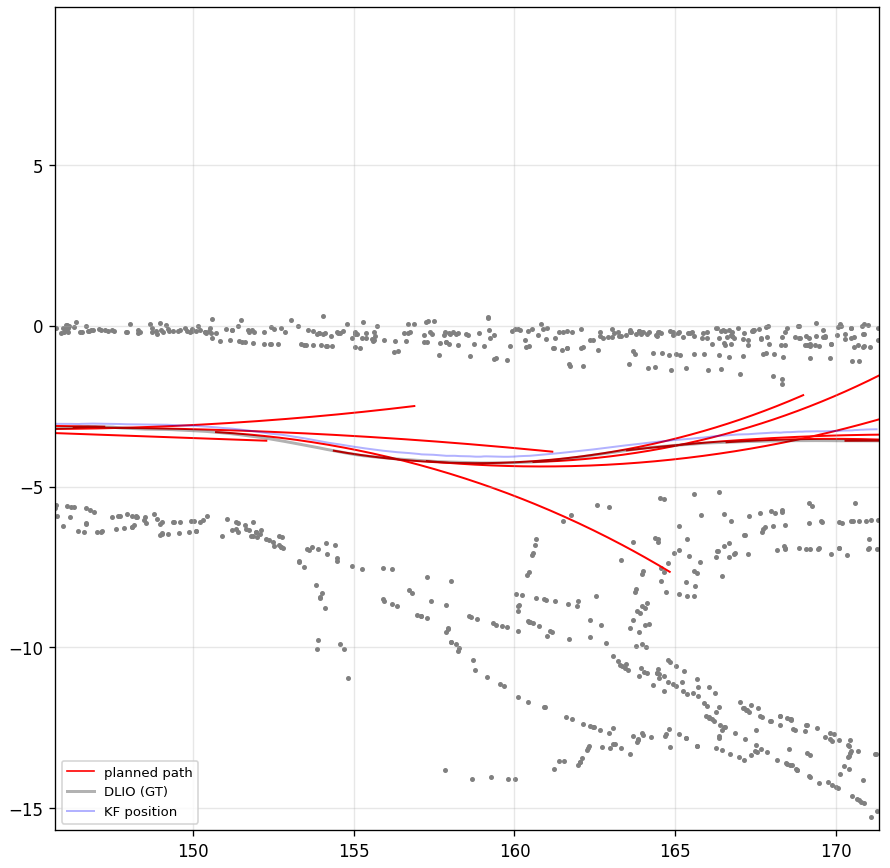
\includegraphics[width=\textwidth]{gambar/fusion_lurus_1.png}
        \caption{Skenario jalan lurus dengan persimpangan}
        \label{fig:fusion_lurus_1}
    \end{subfigure}
    \hfill
    \begin{subfigure}[b]{0.47\textwidth}
        \centering
        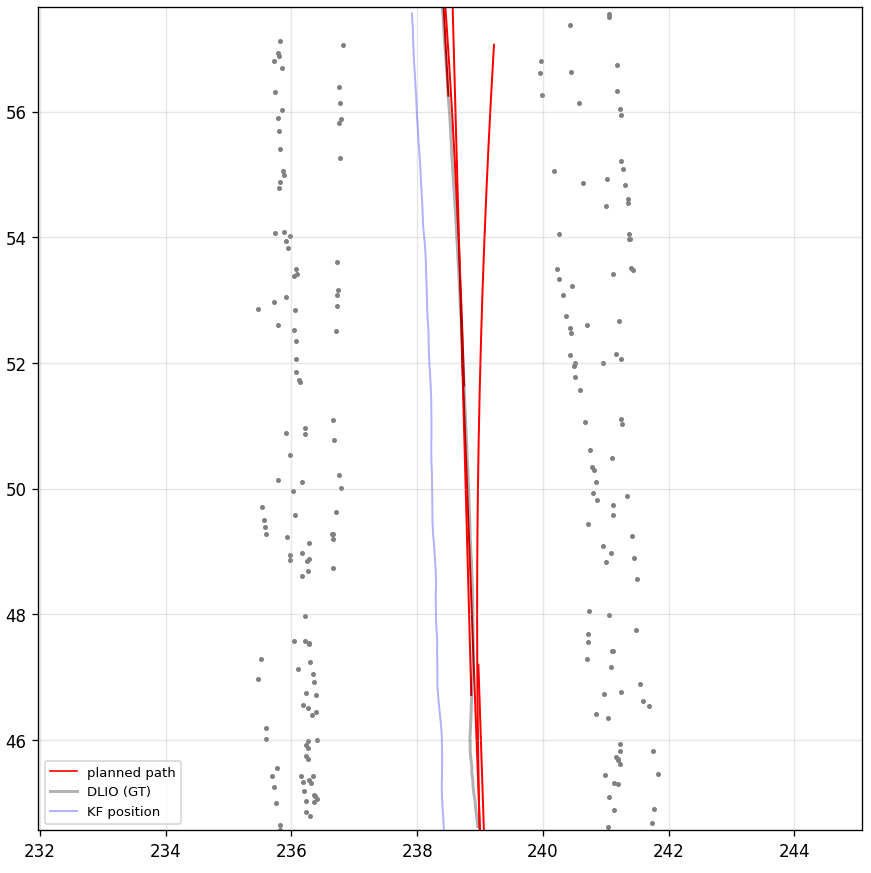
\includegraphics[width=\textwidth]{gambar/fusion_lurus_2.png}
        \caption{Skenario jalan lurus tanpa persimpangan}
        \label{fig:fusion_lurus_2}
    \end{subfigure}
    \caption{Perbandingan lintasan pada skenario jalan lurus dengan persimpangan dan tanpa persimpangan .}
    \label{fig:lurus}
\end{figure}

Pada skenario jalan lurus dengan persimpangan (Gambar~\ref{fig:fusion_lurus_1}), terdapat area putar balik (\emph{H-junction}) di sisi kanan jalan.
Perencanaan lokal berhasil menghasilkan rute di tengah jalan dengan sedikit osilasi pada area putar balik karena target perencanaan lokal yang memaksa kendaraan untuk berada di tengah jalan sedangkan pada area putar balik terdapat celah yang membuat jalan menjadi lebih melebar ke sisi kanan.
Meskipun demikian, perencanaan lokal berhasil melakukan navigasi kendaraan dengan mengikuti arah yang diinginkan dan tetap berada di dalam koridor jalan yang aman.
Sedangkan pada skenario jalan lurus tanpa persimpangan (Gambar~\ref{fig:fusion_lurus_2}), ruas jalan memiliki lebar geometri yang konsisten sepanjang segmen.
Perencanaan lokal berhasil menghasilkan rute di tengah jalan tanpa osilasi sehingga kendaraan dapat mengikuti arah yang diinginkan dengan stabil.

\subsubsection{Manuver Belok}
\label{sec:uji_belok}

Pengujian pada segmen belok dilakukan untuk mengevaluasi performa sistem pada kondisi geometri jalan yang lebih kompleks, yaitu perubahan arah yang signifikan.
Gambar~\ref{fig:belok_1} menampilkan perbandingan lintasan pada dua segmen belok pada lokasi yang berbeda.

\begin{figure}[H]
    \centering
    \begin{subfigure}[b]{0.48\textwidth}
        \centering
        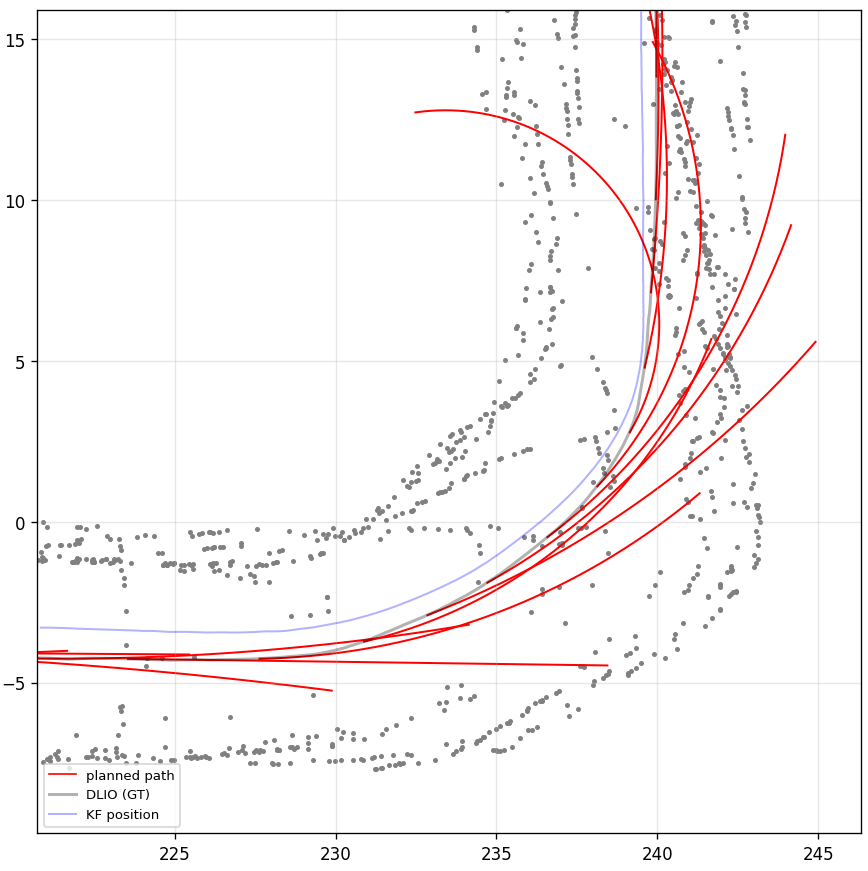
\includegraphics[width=\textwidth]{gambar/fusion_belok_1.png}
        \caption{Skenario belokan 1}
        \label{fig:fusion_belok_1}
    \end{subfigure}
    \hfill
    \begin{subfigure}[b]{0.48\textwidth}
        \centering
        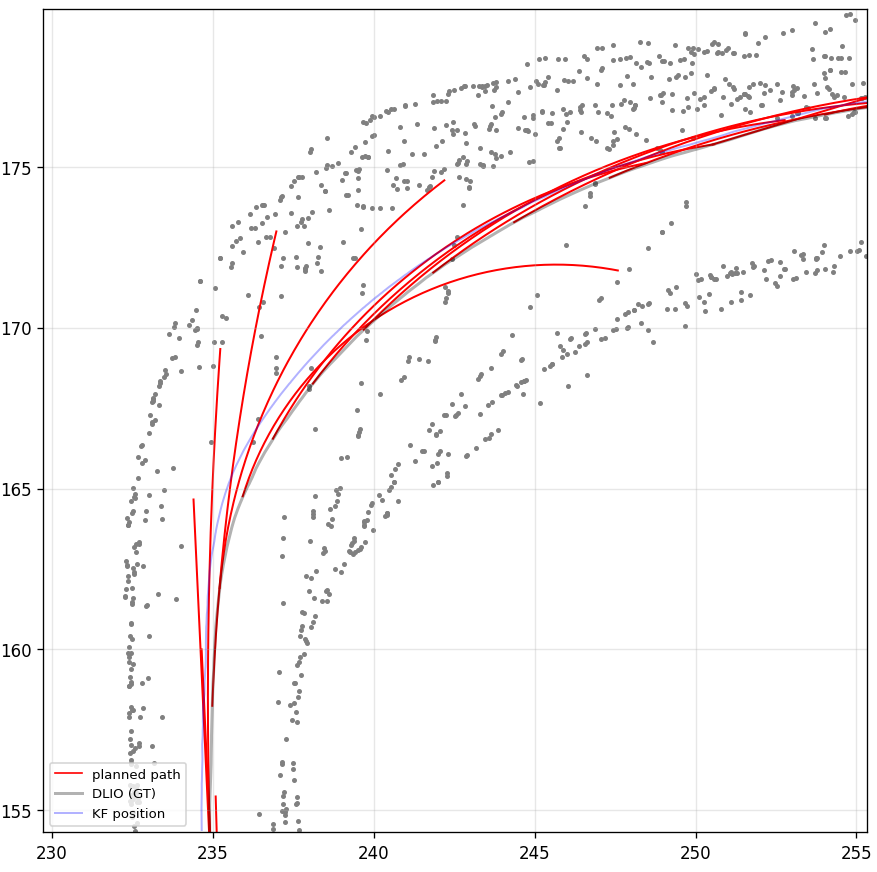
\includegraphics[width=\textwidth]{gambar/fusion_belok_2.png}
        \caption{Skenario belokan 2}
        \label{fig:fusion_belok_2}
    \end{subfigure}
    \caption{Perbandingan lintasan pada skenario yang melibatkan manuver belok pada dua lokasi berbeda.}
    \label{fig:belok_1}
\end{figure}

Pada skenario jalan belok, terdapat dua lokasi dengan radius kelengkungan yang berbeda. Skenario belok 1 memiliki radius kelengkungan yang lebih kecil dibandingkan skenario belok 2, sehingga manuver belok pada skenario belok 1 lebih tajam dan dinamis dibandingkan skenario belok 2 yang memiliki radius kelengkungan lebih besar sehingga manuver belok menjadi lebih halus dan stabil.
Perencanaan lokal berhasil menghasilkan rute yang mengikuti geometri belok pada kedua skenario, meskipun terdapat sedikit osilasi pada skenario belok 1 karena dinamika manuver yang lebih kompleks, tetapi keduanya berhasil membuat kendaraan tetap berada dalam koridor jalan yang aman.

\subsubsection{Manuver Bundaran}
\label{sec:uji_bundaran}

Pengujian pada segmen bundaran dilakukan untuk mengevaluasi performa sistem pada kondisi geometri jalan yang paling kompleks, yaitu perubahan arah yang signifikan dengan radius kelengkungan yang kecil.
Selain itu, pada segmen bundaran terdapat banyak pilihan jalur yang dapat diambil, sehingga perencanaan lokal harus mampu memilih jalur yang sesuai dengan tujuan akhir kendaraan.
Gambar~\ref{fig:bundaran} menampilkan perbandingan lintasan pada segmen bundaran dengan putaran 90\textdegree dan 180\textdegree terhadap lintasan yang dihasilkan oleh perencanaan lokal.

\begin{figure}[H]
    \centering
    \begin{subfigure}[b]{0.48\textwidth}
        \centering
        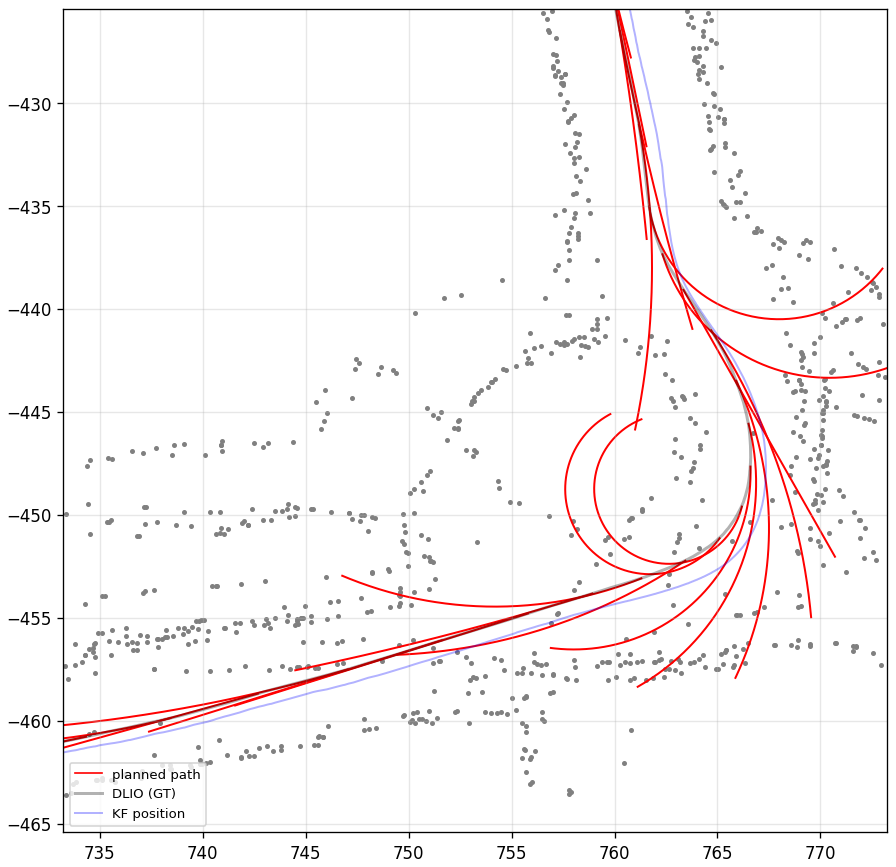
\includegraphics[width=\textwidth]{gambar/fusion2_bundaran_1.png}
        \caption{Skenario bundaran dengan putaran 90\textdegree}
        \label{fig:bundaran_1}
    \end{subfigure}
    \hfill
    \begin{subfigure}[b]{0.48\textwidth}
        \centering
        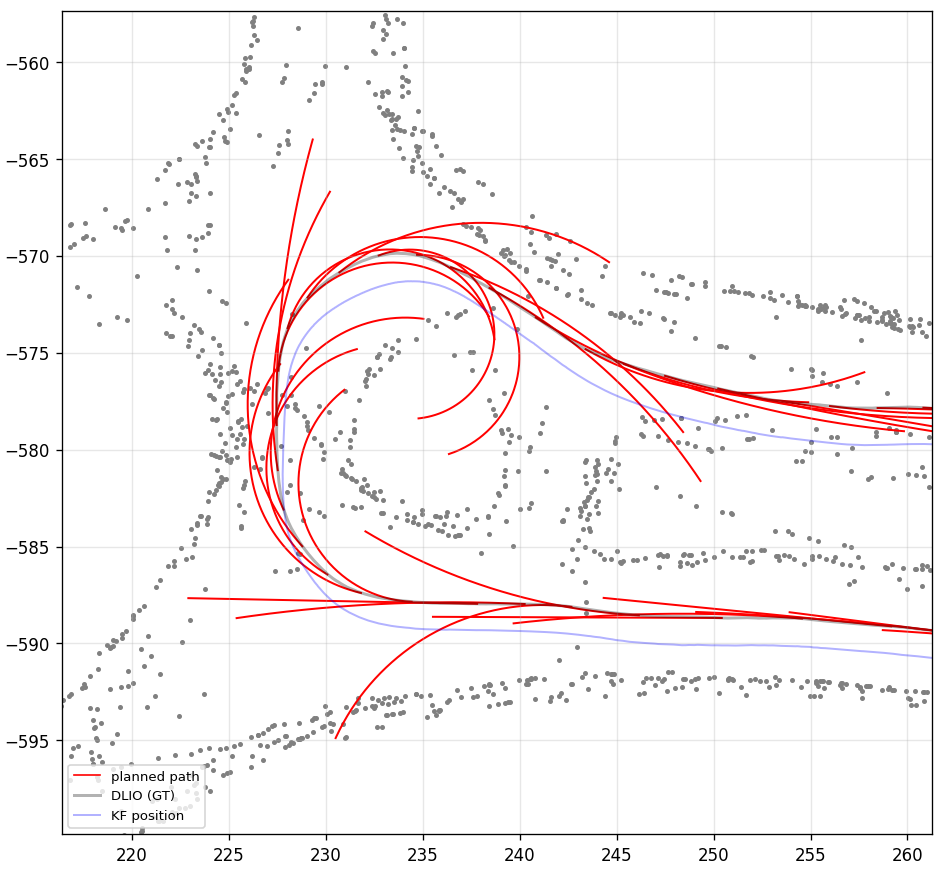
\includegraphics[width=\textwidth]{gambar/fusion2_bundaran_2.png}
        \caption{Skenario bundaran dengan putaran 180\textdegree}
        \label{fig:bundaran_2}
    \end{subfigure}
    \caption{Perbandingan lintasan pada skenario yang melibatkan manuver bundaran dengan putaran 90\textdegree (Gambar~\ref{fig:bundaran_1}) dan 180\textdegree (Gambar~\ref{fig:bundaran_2}).}
    \label{fig:bundaran}
\end{figure}

Pada skenario bundaran dengan putaran 90\textdegree (Gambar~\ref{fig:bundaran_1}), perencanaan lokal berhasil menghasilkan rute yang mengikuti geometri bundaran dengan baik dan mampu memilih rute belok ke kanan yang sesuai dengan tujuan akhir kendaraan.
Begitu juga pada skenario bundaran dengan putaran 180\textdegree (Gambar~\ref{fig:bundaran_2}), perencanaan lokal berhasil menghasilkan rute yang mengikuti geometri bundaran dengan baik dan mampu menghasilkan rute putar balik yang sesuai dengan tujuan akhir kendaraan.
Meskipun kedua perencanaan lokal mengalami cukup banyak osilasi pada area bundaran, namun keduanya berhasil membuat kendaraan tetap berada dalam koridor jalan yang aman dan mampu mengikuti arah yang diinginkan dengan baik.